\subsection{RQ1: conflicts and additional alarms}\label{sec:rq1}

We report detection counts alongside the additional findings that a reviewer would need to assess. Conflict alarms are counts of runs, ambiguity flags are counts of rules, and the scale observations are individual measurements.

E18 used six new domains---beds, timesheets, aquariums, cloakrooms, turbines and
payroll---with six versions each: clean, direct conflict, overlapping conflict,
two ambiguities, and a gap. The set was committed before the design was frozen.
The 108 runs contain 36 planted conflict opportunities and 18 clean runs.
The comparison in Table~\ref{tab:e18} scores the \emph{same saved runs} with and
without the facts added by the outcome-pair questions. It therefore isolates
that addition without resampling the earlier formalization.

\begin{table}[H]
\centering
\small
\begin{tabularx}{\linewidth}{@{}Xrr@{}}
\toprule
E18 measure & Without questions & With questions \\
\midrule
Planted conflicts found & 27/36 & 34/36 \\
\quad Direct conflicts & 9/18 & 16/18 \\
\quad Overlapping conflicts & 18/18 & 18/18 \\
Clean runs with a conflict alarm & 0/18 & 3/18 \\
Unexpected conflicts, all versions & 1 & 28 \\
Planted ambiguities found & 16/36 & 16/36 \\
Planted gaps found & 17/18 & 17/18 \\
Clean runs with a gap on a covered event & 0/18 & 0/18 \\
\bottomrule
\end{tabularx}
\caption{E18: default scoring, including doubtful conflicts. Removing doubtful
conflicts changes unexpected-conflict counts to 0 and 27; the other entries
are unchanged. Counts of findings and counts of runs are distinct.}
\label{tab:e18}
\end{table}

\begin{figure}[H]
\centering
\begin{minipage}{0.48\linewidth}
\centering
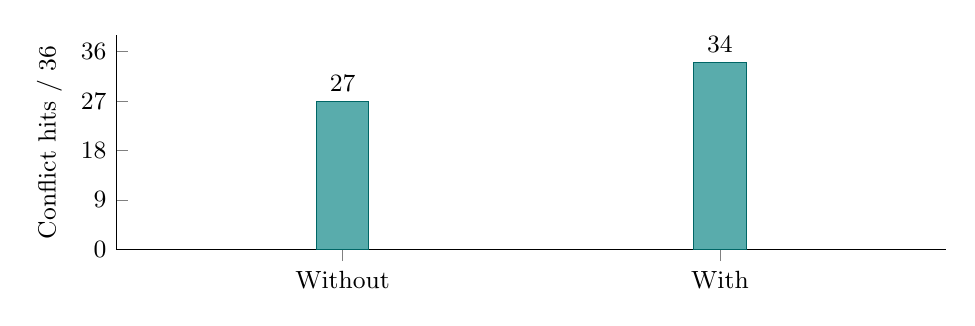
\begin{tikzpicture}
\begin{axis}[width=\linewidth,height=4.3cm,ybar,bar width=19pt,
  ymin=0,ymax=39,ytick={0,9,18,27,36},xmin=-0.6,xmax=1.6,
  xtick={0,1},xticklabels={Without,With},
  ylabel={Conflict hits / 36},tick label style={font=\small},
  label style={font=\small},nodes near coords,
  every node near coord/.append style={font=\small},
  axis lines*=left,enlarge x limits=false]
\addplot[fill=teal!65,draw=teal!80!black] coordinates {(0,27) (1,34)};
\end{axis}
\end{tikzpicture}
\end{minipage}\hfill
\begin{minipage}{0.48\linewidth}
\centering
\begin{tikzpicture}
\begin{axis}[width=\linewidth,height=4.3cm,ybar,bar width=19pt,
  ymin=0,ymax=19.5,ytick={0,3,6,9,12,15,18},xmin=-0.6,xmax=1.6,
  xtick={0,1},xticklabels={Without,With},
  ylabel={Clean alarm runs / 18},tick label style={font=\small},
  label style={font=\small},nodes near coords,
  every node near coord/.append style={font=\small},
  axis lines*=left,enlarge x limits=false]
\addplot[fill=orange!65,draw=orange!80!black] coordinates {(0,0) (1,3)};
\end{axis}
\end{tikzpicture}
\end{minipage}
\caption{The E18 tradeoff. ``With'' means the outcome-pair questions are
included. Each axis states its own denominator; these are different measures.}
\label{fig:e18-tradeoff}
\end{figure}

\example{A conflict recovered: releasing and holding a hospital bed}
The original translation used separate symbols for releasing a bed and holding
it for 24 hours. Z3 could satisfy both. All eight answers to the outcome
question judged them incompatible, supplying the missing assumed fact. The
planted conflict was then found in all three runs. Retention wording in the
cloakroom case was similarly recovered. Across E18, 410 pairs were asked about
and 58 received a majority of ``impossible'' answers.
\source{research_log.md, E18; experiments/results/E18_eval12.json}

\example{A conflict still missed: retaining payroll records}
``Keep every payslip for ten years'' sometimes became merely
\code{payslip_retention_years = 10}. Nothing in that formula prevents deletion.
One run supplied the missing connection, another split four votes to four,
and a third expressed conditional retention rather than one definite outcome,
so the pair was not asked about. The direct payroll conflict was found in only
one of three runs. More samples do not automatically repair the choice of symbols.

\example{The cost: collecting a coat that was previously unclaimed}
A clean cloakroom specification says to release a coat when a guest presents
its token, and to list coats left for over 30 days as unclaimed. The one-snapshot
model treats release and being unclaimed as incompatible simultaneous outcomes.
A perfectly ordinary history---list the coat first, release it later---has been
collapsed. This one pair accounts for 24 of the 27 additional unexpected
conflicts across versions, including all three clean-run alarms. The remaining
three additional findings involve a planted timesheet rule and a third rule.
The unexpected findings therefore need individual review. In the cloakroom
case, the alarm comes from collapsing successive states into one snapshot.
\source{research_log.md, E18; experiments/results/E18_eval12.md}

The earlier T22 development-data ablation supports the same tradeoff: on saved
models from eight older sets, conflict hits rose from 132/153 to 145/153.
With doubtful findings excluded, the corresponding values were 129/153 and
142/153, while clean alarm runs rose from 3/144 to 13/144. Those results
motivated the design; they remain separate from the held-out E18 evidence.
\source{research_log.md, T22}

\subsection{RQ2: ambiguity and review questions}\label{sec:rq2}

\begin{table}[H]
\centering
\small
\begin{tabular}{@{}lrr@{}}
\toprule
Measure & Main model & With second reader \\
\midrule
E9: planted ambiguities & 14/36 & 30/36 \\
E9: clean-spec rule flags (18 runs) & 7 & 15 \\
E12: planted ambiguities & 17/36 & 32/36 \\
E12: clean-spec rule flags (18 runs) & 5 & 9 \\
\bottomrule
\end{tabular}
\caption{Second-reader results on two separate 72-run experiments. Rule flags
are counts, not percentages of clean runs.}
\label{tab:second-reader-evaluation}
\end{table}

\example{Does ``if'' govern the gate, the photograph, or both?}
The ski-pass example requires the system to ``open the gate and show the
skier's photo if the pass is a season pass''. A reader can attach the condition
to the photograph alone or to both actions. A second model is more likely to
disagree with the first model's confident choice. Table~\ref{tab:second-reader-evaluation}
shows the resulting gain, together with additional review work. The clean-spec
flags are unplanted ambiguities whose correctness has not been independently
labelled, so we cannot count them all as false positives.
\source{experiments/sets/eval7/skipass_ambiguity2/spec.md; experiments/results/E9_eval4.md; experiments/results/E12_eval7.md}

\subsection{RQ3: changes and reuse}\label{sec:rq3}

E17 evaluates a different question: can the system apply an OpenSpec change,
preserve scenario identity, and report findings involving that change? Across
90 runs it found all 36 planted conflicts and all 36 planted gaps, with no
unexpected conflict or covered-event gap reported about the 18 clean changes.
Excluding doubtful conflicts reduces the conflict count to 33/36. All 90 runs
preserved the generated scenario labels.

\example{A cinema change stops seat sales when the projector fails}
The change modifies the operations specification to prohibit sales while a
hall's projector is out of order. The existing screenings specification still
requires a sale when a customer requests an available seat. Checking the merged
document exposes that interaction across files. In all three runs, however,
the projector's state was modelled as an event, making the conflict doubtful.
Filtering doubtful findings therefore loses this planted case.

The conflict wording in E17 deliberately negates an existing outcome directly.
The results support merging, labels and finding selection; they leave harder
semantic translations untested. At the time, removal-only gaps were not attributed to their
change, every scenario under a modified requirement counted as changed, and each
change required full formalization. E19 and E20 evaluate later changes to those behaviours.
\source{experiments/results/E17_eval11.md; research.md, sections 2.4 and 4.5}

\paragraph{E19: removals and unchanged scenarios.}
The next six projects contain 36 changes, each run three times. These cases include removing a whole requirement, dropping a scenario, narrowing coverage, retiring an event, and modifying one scenario while leaving its siblings unchanged. Table~\ref{tab:e19} separates the planted defects from quiet changes. The 54 quiet-change runs include clean, retirement and unchanged-sibling cases; their denominator differs from E17's 18 clean runs.

\begin{table}[H]
\centering
\small
\begin{tabularx}{\linewidth}{@{}Xr@{}}
\toprule
E19 measure & Result \\
\midrule
Planted conflicts found & 18/18 \\
\quad After excluding doubtful findings & 15/18 \\
Planted gaps found & 35/36 \\
\quad Whole-requirement removals & 18/18 \\
\quad Dropped scenarios or narrowed coverage & 17/18 \\
Quiet-change runs with a conflict alarm & 2/54 \\
Quiet-change runs with a gap alarm & 0/54 \\
Runs preserving scenario labels & 108/108 \\
\bottomrule
\end{tabularx}
\caption{E19: removal handling and more precise scenario provenance.}
\label{tab:e19}
\end{table}

All eighteen event-retirement runs stayed quiet. Existing conflicts were found and excluded from the change report in all 108 run opportunities, covering six distinct old conflicts. In the missed narrowed-coverage case, the translation of a retained rule lost a condition and appeared to cover the missing branch. The two quiet-change conflict alarms involved reworded scenarios: textual change tracking cannot establish that a rewrite has the same meaning. These results support the new attribution mechanism on the tested cases, not complete regression detection.
\source{experiments/results/E19_eval13.md; research_log.md, E19}

\paragraph{E20: full formalization versus a saved base.}
E20 uses six further projects and 36 distinct changes, with three repetitions per mode. Each repetition includes eighteen planted-conflict, twelve planted-gap and six clean changes. The full mode chooses a vocabulary and translates the combined document; reuse keeps the base vocabulary and readings and translates the changed scenarios. Both then run the ordinary solver checks on their resulting encodings.

\begin{table}[H]
\centering
\small
\begin{tabularx}{\linewidth}{@{}Xrr@{}}
\toprule
E20 measure & Full & Reuse \\
\midrule
Planted conflicts found & 54/54 & 50/54 \\
\quad After excluding doubtful findings & 51/54 & 45/54 \\
Planted gaps found & 36/36 & 36/36 \\
Clean-change runs with conflict or gap alarms & 0/18 & 0/18 \\
Other change-related conflicts & 3 & 1 \\
Unplanted ambiguity flags & 1 & 4 \\
All change-related gaps & 39 & 42 \\
Runs preserving scenario labels & 108/108 & 108/108 \\
\bottomrule
\end{tabularx}
\caption{E20: detection changes when a saved interpretation is reused. Clean-run quietness does not mean that every other finding was a planted defect.}
\label{tab:e20}
\end{table}

\example{A new rule is read with a narrower trigger.}
In the driving-school case, a new rule about a person younger than seventeen sometimes acquired an unspoken registration-event condition when translated against the saved base. Disagreement or selection of a non-conflicting reading then lost the planted overlap conflict. The four missed run opportunities concern two distinct changes: this case in all three repetitions, and a brewery conflict in one. Reusing the base saves translation work but can alter how the new text is understood. The request savings are reported under RQ4; these data do not establish equal accuracy between the modes.
\source{experiments/results/E20_eval14_full.md; experiments/results/E20_eval14_incremental.md; research_log.md, E20}

\subsection{RQ4: scale and cost}\label{sec:rq4}

\paragraph{Requests saved by reusing a base.}
E20 recorded the API requests and tokens used by the formalization stage. The measurements exclude the CLI's later explanation and scenario-judging calls. Table~\ref{tab:reuse-cost} separates the initial base build from each subsequent change.

\begin{table}[H]
\centering
\small
\begin{tabularx}{\linewidth}{@{}Xrrr@{}}
\toprule
Mean formalization usage & Full change & Reused-base change & Initial base \\
\midrule
API requests & 68 & 9 & 61 \\
Prompt tokens & 32,431 & 4,934 & 28,641 \\
Completion tokens & 28,806 & 3,816 & 25,969 \\
\bottomrule
\end{tabularx}
\caption{E20: rounded means. The base cost is additional and can be shared only while that base remains reusable. One request can return eight samples.}
\label{tab:reuse-cost}
\end{table}

The recorded totals were 7,336 requests for full runs, 1,010 for changes using saved bases, and 1,093 for eighteen base builds. Including those builds, reuse used 2,103 requests, about 71\% fewer in this experiment with six alternative changes per base. Excluding base builds gives about 86\% fewer. Neither percentage is an end-to-end CLI cost or a monetary saving. Archiving a change into the base forces a new build; one check after each archive therefore has a different cost profile. A removal-only change may need no new formalization calls while still requiring LLM calls to explain its findings.

The recorded batch times were about 32 minutes for full mode and 13 minutes for reuse including bases. These are observations from one batch setup, not per-change latency estimates. The conflict-detection loss in Table~\ref{tab:e20} is part of the same comparison and should accompany the savings.
\source{experiments/results/E20_eval14_full.md; experiments/results/E20_eval14_incremental.md; experiments/evaluate.py; research_log.md, E20}

\paragraph{Larger specifications.}

For the 30-requirement campsite document, skipping combinations from unrelated
rule families reduced solver time from 26--34 seconds to 0.4--0.9 seconds on
the saved models. Booking, barriers, showers and billing share few symbols.
Both planted conflicts were found in all three repetitions, as was the gap.
Each clean run had a doubtful conflict; excluding doubtful findings left none.
A densely connected document need not obtain the same speedup.

The 100-requirement ferry example required a larger read-output allowance:
one measured answer contained 16,799 tokens. All 12 runs then read the correct
number of requirements in their respective variants. Conflict hits were 6/6,
gap hits 3/3, and one of three clean runs had a conflict alarm. The culprit was
reserving a new seat versus releasing an old unpaid reservation: one state
variable represented different seats at different times. As in the cloakroom
example, the representation fails to distinguish states at different times;
here it also conflates separate objects.

One 101-rule model took 35 seconds in the solver; one full CLI run including
wording took 620 seconds on a busy cluster server. These are observations,
not latency averages. E18's 24 minutes for 108 runs on two GPUs is a separate
batch-throughput measurement. The current second-reader server cannot fit the
long ferry prompt under its configured prompt-plus-answer allowance, and the
outcome check asks only the first 40 eligible pairs on large documents.
\source{research_log.md, E13, E14 and E18}

